\documentclass[11pt,letterpaper]{article} % for a short document

% Bibliography
\usepackage[authordate,strict,autolang=hyphen,bibencoding=inputenc,doi=true,isbn=false,annotation=false]{biblatex-chicago}
\usepackage{graphicx}
\DeclareGraphicsExtensions{.pdf,.png,.jpg}
\usepackage[section]{placeins}
\addbibresource{../references/references.bib}
\usepackage{booktabs}

\title{Reproducible Sausage Buffers for Urban Form Analysis: A Case Study of PostGIS}
\author{Phil Hurvitz, \ldots}
\date{}

%%% BEGIN DOCUMENT

\begin{document}

\maketitle

\section*{Background}
When delineating travel catchment areas or travel sheds, network-based
buffers are often preferable to circular, great arc buffers in that
network buffers more realistically reflect the distance limitations
imposed by different street patterns. \textcite{Forsyth2014sausage}
identified a threat to replicability for studies using such
network-based buffers, due to changes over the years in how ESRI's
market-leading GIS software has calculated them. In response,
\citeauthor{Forsyth2014sausage} proposed ``sausage'' network buffers,
created via a transparent algorithm, for use in measuring aspects of
urban form related to food and physical activity. Presented as
replicable and cross-platform, the implementation described in that
article nevertheless relies on ESRI's commercial GIS and Network
Analyst extensions, and is thus tied to the Microsoft Windows
platform. Their paper called on others to validate sausage buffers
created via other GIS software on other platforms. This paper answers
that call, validating the the sausage buffer technique with particular
attention paid to reproducibility and cross-platform implementation
using readily available free and open source software.

% Let's mention something about reproducibility up front.
The methods presented here are also in part a response to a growing
call from across numerous disciplines to ensure computer aided
analyses are reproducible. The basic standard for reproducibility is
that the data used are available, and that analyses are shared in the
form of computer code \cite{Peng2011computational}. In that sense, the
methods presented here are reproducible because analyses are fully
automated using computer code, rather than being reliant on a set of
manual procedures. Those pieces of code and the data are publicly
available.\footnote{need to package up code and data, upload to UW's
  repository, and then see about generating a DOI.}  Further, building
these methods atop free and open source software achieves a higher
standard of reproducibility by eliminating dependencies on any ``black
box'' computer code. In principle, this means that every piece of
software used in these methods is open to scrutiny.

% Relevance to planning and epidemiology
Developing geoprocessing methods around free and open source tools
holds particular benefits for disciplines such as epidemiology, public
policy, and urban planning because of the reduced barriers of adoption
for practitioners and advocates outside of academia. Academic
institutions and larger public agencies may be able to afford software
licenses. However, smaller agencies or advocacy groups wishing to
perform this type of walkshed analysis might otherwise be unable to
make use of analyses reliant on proprietary software simply due to the
cost of software licenses.

% Not a literature review, per se. Since we are developing a methods
% paper largely in response to one particularly important method, I'm
% not sure how important a full-blown review is. Open to suggestions,
% however. This could potentially be split off and developed into
% something more complete. 
Finally, the PostGIS platform is especially beneficial in that it
naturally facilitates reproducible, scripted analyses, as well as can
provide the core infrastructure for data management on a research
project. \textcite{hurvitz2014emerging} describe the use of
PostgreSQL/PostGIS to manage and process geospatial and timeseries
data from a variety of sources including GPS and
accelerometers. However, we are neither first nor alone in identifying
PostGIS for use in research. In a keyword search for ``PostGIS'' using
ISI Web of Science, we identified 35 articles across a number of
disciplines describing the use of PostGIS in research. In the
transportation sector, \textcite{Wang2015routable} also used PostGIS
to store and analyze a large number of GPS traces in order to infer
characteristics about roadways such as position and rules, for the
purposes of generating routable roadway networks. In another recent
article, \textcite{Brovelli2015FOSS} describe the use of PostGIS
together with GeoServer to collect data about roadway pavement
conditions from the general public. Notable in this study is the
potential for PostGIS in supporting digitally-mediated public
participation.



\section*{Methods}
% Set-up and software PgRouting 2.x on OpenBSD 5.7 i5
In this section we describe how, following the process described by
\textcite{Forsyth2014sausage, Forsyth2012proto}, we implemented the
sausage buffering technique using the PostgreSQL relational database
with PostGIS and PgRouting extensions. Using that technique we
generated 200 such buffers around randomly selected points. We then
compare those results to buffers analogously created in ArcGIS Desktop
10.2.X, for use as a basis for comparison with the results presented
by \citeauthor{Forsyth2014sausage}. Table \ref{tab:software} lists
software versions used in this analysis.


\begin{table}[h!]
  \centering
  \caption{Software used to generate PostGIS and ESRI sausage buffers}
  \begin{tabular}{llr}
  \toprule
  Buffer type & Software & Version \\
  \midrule
PostGIS/PgRouting & OpenBSD (Operating System) & 5.7 \\
              & PostgreSQL & 9.4.2 \\
              & PostGIS Extensions & 2.1.7 \\
              & PgRouting & 2.0.0 \\
              & Osm2pgrouting & 2.0.0 \\
              &  &  \\
  ESRI & Microsoft Windows & Eric? \\
              & Arc(Map)? & 10.2.X Eric? \\
  \bottomrule
\end{tabular}
\label{tab:software}
\end{table}

In overview, the process for creating a sausage buffer entails three
key steps. First, a point of origin is identified on a network of
transportation facilities. Next, a distance threshold is selected. The
network is traversed outward along all possible paths from the point
of origin until reaching the distance threshold. The resulting subset
reflects portions of the network reachable within the chosen
distance. Finally, the segments of the network subset are buffered
according to some chosen buffer radius, resulting in a set of polygons
reminiscent of sausages. These are combined into a single polygon,
forming the final buffer. Figure \ref{fig:sausage-steps} illustrates
these steps.

\begin{figure}[h!]
  \centering
  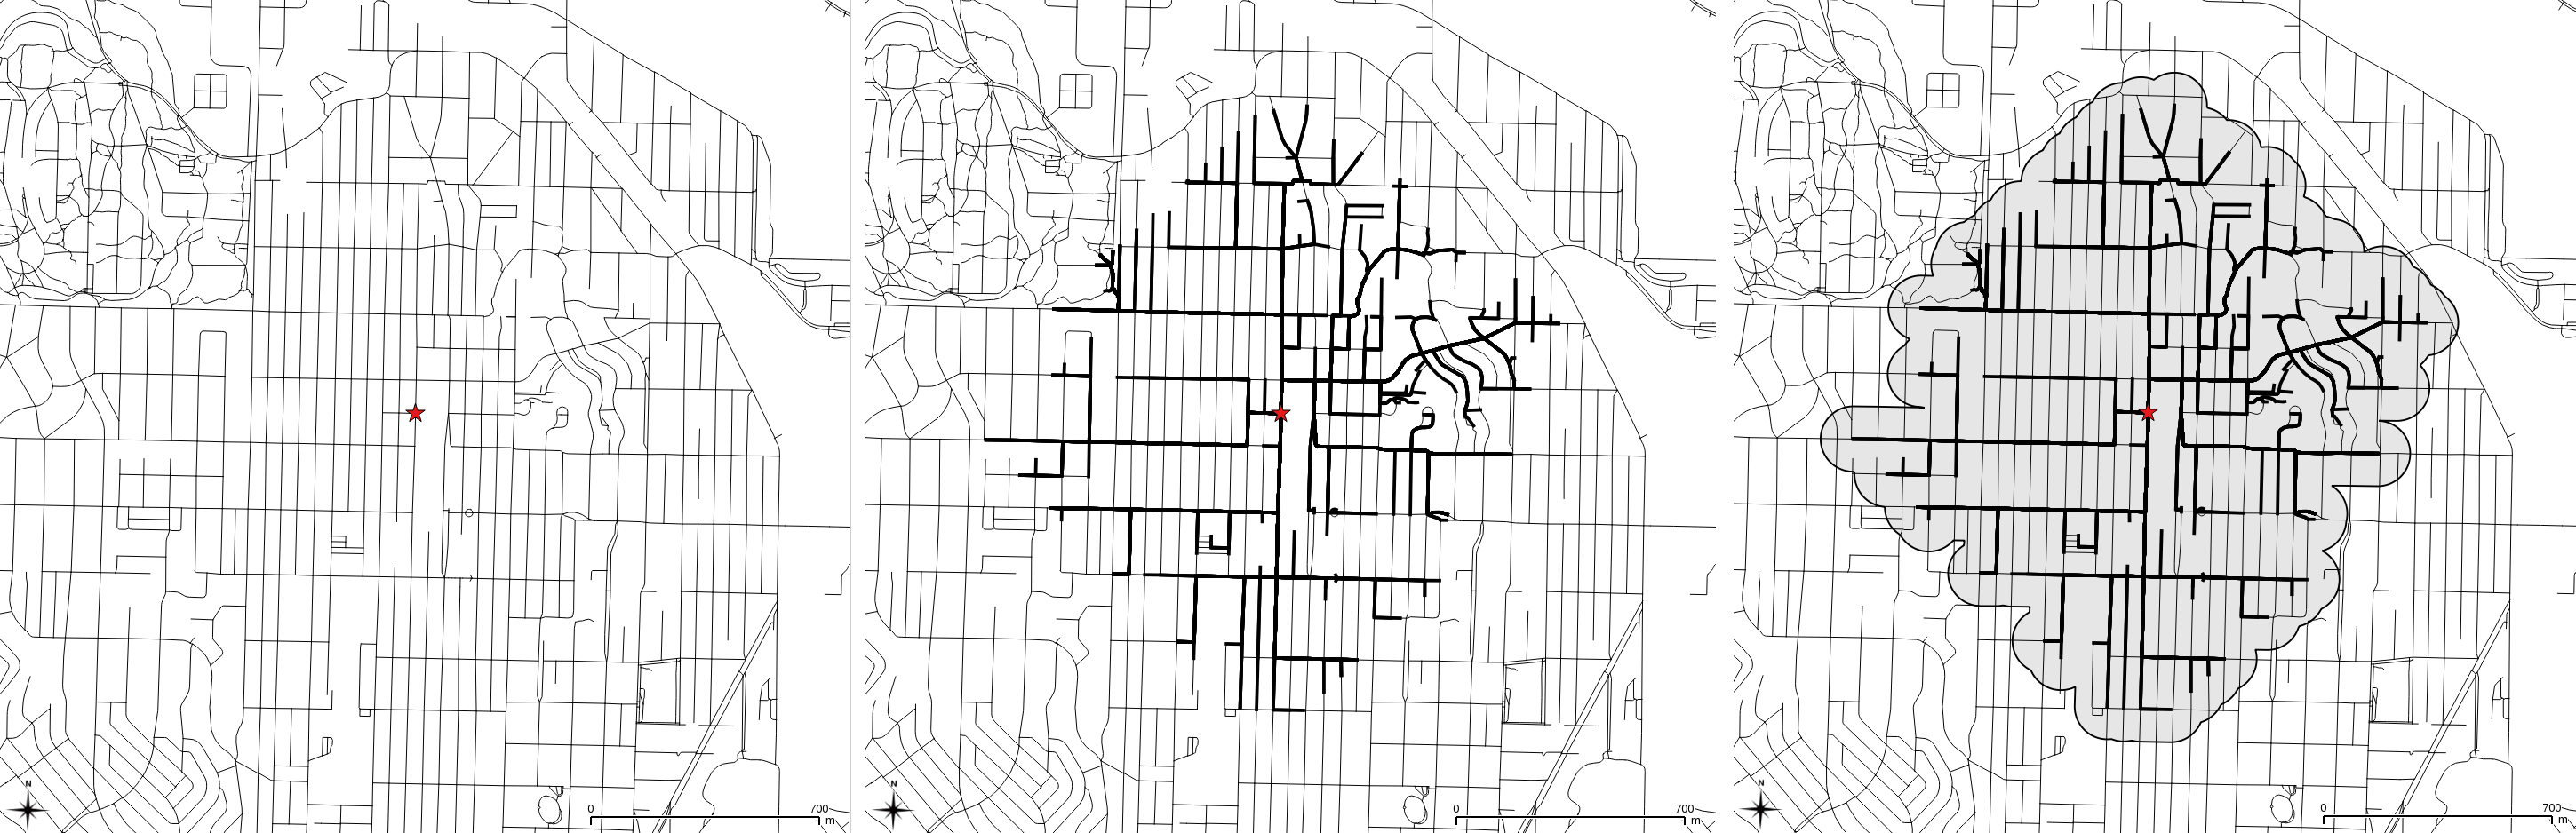
\includegraphics[width=\textwidth]{./figs/sausage-steps}
  \caption{From left to right, the three primary steps in creating a
    sausage buffer. First, an origin is selected. Next, the portions
    of the network reachable within a given distance threshold (here,
    1km) are identified. Finally, lines are combined and buffered.}
  \label{fig:sausage-steps}
\end{figure}

%\subsection*{Data sources and network import}
To create the routable network required for generating the buffers, we
imported the Washington State portion of the Open Street Map (OSM)
into PostGIS / PgRouting using the open source osm2pgrouting
utility. Because much of our work deals with pedestrian travel, we
excluded highway facilities, which often do not allow for pedestrian
access. The osm2pgrouting import strategy yielded two primary
benefits. First, osm2pgrouting facilitates reproducible data
importation through the use of an XML-based configuration file. This
allows facility exclusions, such as our exclusion of highways for
pedestrians, to be carried out consistently. Secondly, this strategy
preserves the topology of the OSM network, rather than inferring a
topology from the network's geometry. This second point has
implications for comparability of buffers that we will discuss later.

%\subsection*{Generation of buffers}

% Creation of buffer code in database
% Random sample of 200 vertices as points to construct buffers around
% Define sausage buffering procedure in PLSQL
% Construct 1000m buffer (net dist), 100m (arc dist)
% Rounded versus squared ends
We then implemented the sausage buffering algorithm in the PL/PgSQL
programming language, which is an extended variant of the SQL
programming language. This allowed us to define the sausage buffering
procedures and then store them together with data in the
database. Here, we defined two such functions. The first calculates a
single sausage buffer around a single point of origin. The second uses
the first function to calculate sausage buffers around an arbitrary
number of points.

Because a point of origin may not be located precisely on the network,
the sausage buffering function begins by identifying the nearest
vertex in the network to the identified point of origin. To limit the
required number of distance calculations required, the function then
identifies vertices within a circular buffer with radius equal to the
chosen network distance threshold. This buffer represents the maximum
possible distance one could travel on the network in any given
direction. We then calculate the distance to each vertex within this
circular buffer, discarding routes exceeding the distance threshold,
and retaining those less than or equal to the threshold.\footnote{We
  believe this approach to be computationally inefficient, however
  necessary due to the lack of a built-in service area function in
  PgRouting. Our hope is that future versions of PgRouting will
  include service area analysis, thus simplifying and speeding up
  creation of these buffers.} The resulting set of lines are then
buffered according to the buffer radius, and the resulting polygons
are dissolved into a single geometry.

After implementing the sausage buffering technique in PL/PgSQL, we
then used it to generate buffers originating from 200 randomly
selected points. To ensure that these points were not located in
roadless areas of the state, we selected these points from the
vertices in the roadway network. Then, in order to compare buffers
created using our implementation with buffers described in the
original \citeauthor{Forsyth2014sausage} paper, we created buffers
around the same set of 200 points using the protocols described in
\textcite{Forsyth2012proto}, with one change. In that document, the
protocols call for ``flat'' ended buffers, however in the more
recently published article, \citeauthor{Forsyth2014sausage} describe
rounded buffer ends. We chose to implement the rounded buffer ends as
we believe they are more theoretically defensible.

We carried out this process of duplication manually as described in
that document using ArcGIS 10.X. In addition, to ensure a maximum of
consistency between the datasets used to generate buffers, we exported
both the random points as well as the road network. We exported both
of these datasets as shapefiles, which were then imported into
ArcGIS. Worth noting is that, as described in the
\textcite{Forsyth2012proto} protocols and replicated by us, the
roadway network was imported without preserving the original OSM
topology. While we believe the resulting networks to be largely the
same, we note it as a potential source of difference in the two
analyses.

Finally, we made two cross-comparisons between the two sets of
buffers. Here we matched pairs of buffers according to a unique
identifier assigned to the initial set of points. First we compared
the areas of the two sets of buffers. To assess whether differences in
the areas between these two groups were statistically significant, we
used a Bayesian procedure somewhat analogous to a t-test called BEST
\autocite{Kruschke2014,Kruschke2013}. Second, to assess the possibility of
spatial misalignment between similarly sized buffers, we computed the
symmetric difference of the two sets of sausage buffers and then
calculated the area of the non-overlapping regions. The results of
these comparisons are presented in the following section.


\section*{Results and Discussion}
On comparing the areas of the two sets of sausage buffers, we found
that, overall, they were very similar, with perhaps more
PostGIS-generated buffers at slightly smaller sizes. Figure
\ref{fig:area_dens} shows the distribution of these two sets of
buffers. Both exhibit the same somewhat bimodal shape, with greater
differences observed among smaller buffers. 

That apparent difference in size did not, however, constitute a
statistically significant difference between the two sets of
buffers. We estimated the mean difference's 95\% confidence interval
as ranging from -.23 to 0.04. Because a mean difference of zero falls
within our 95\% confidence interval, we cannot say for certain that
PostGIS generated sausage buffers will generally be smaller than
buffers created in ArcGIS.

\begin{figure}[h!]
  \centering
  \includegraphics[width=0.65\textwidth]{../results/area_dens}
  \caption{Density plot showing the distributions PostGIS- and
    ESRI-generated sausage buffers across the range of sizes.}
  \label{fig:area_dens}
\end{figure}

When we compare the symmetric differences between the two sets of
buffers we see (figure \ref{fig:symdiff_dens}) that most of these
regions are small. Figure \ref{fig:symmetric_differences} illustrates
three scenarios including the best, typical (closest to the median),
and worst cases with respect to these symmetric differences. In the
best case, we see that the buffers encompassing a very small, isolated
pedestrian facility are practically identical. In the more typical
case, slight differences are visible upon close inspection. Finally,
in the worst case, which was located in a remote portion of Central
Washingtion, it is apparent that the buffers are very different, with
the PostGIS buffer only a subset of the larger ESRI-generated buffer.

\begin{figure}[h!]
  \centering
  \includegraphics[width=0.65\textwidth]{../results/symdiff_dens}
  \caption{Density plot showing the distribution of symmetric
    differences between PostGIS- and ESRI-generated sausage buffers.}
  \label{fig:symdiff_dens}
\end{figure}

\begin{figure}[h!]
  \centering
  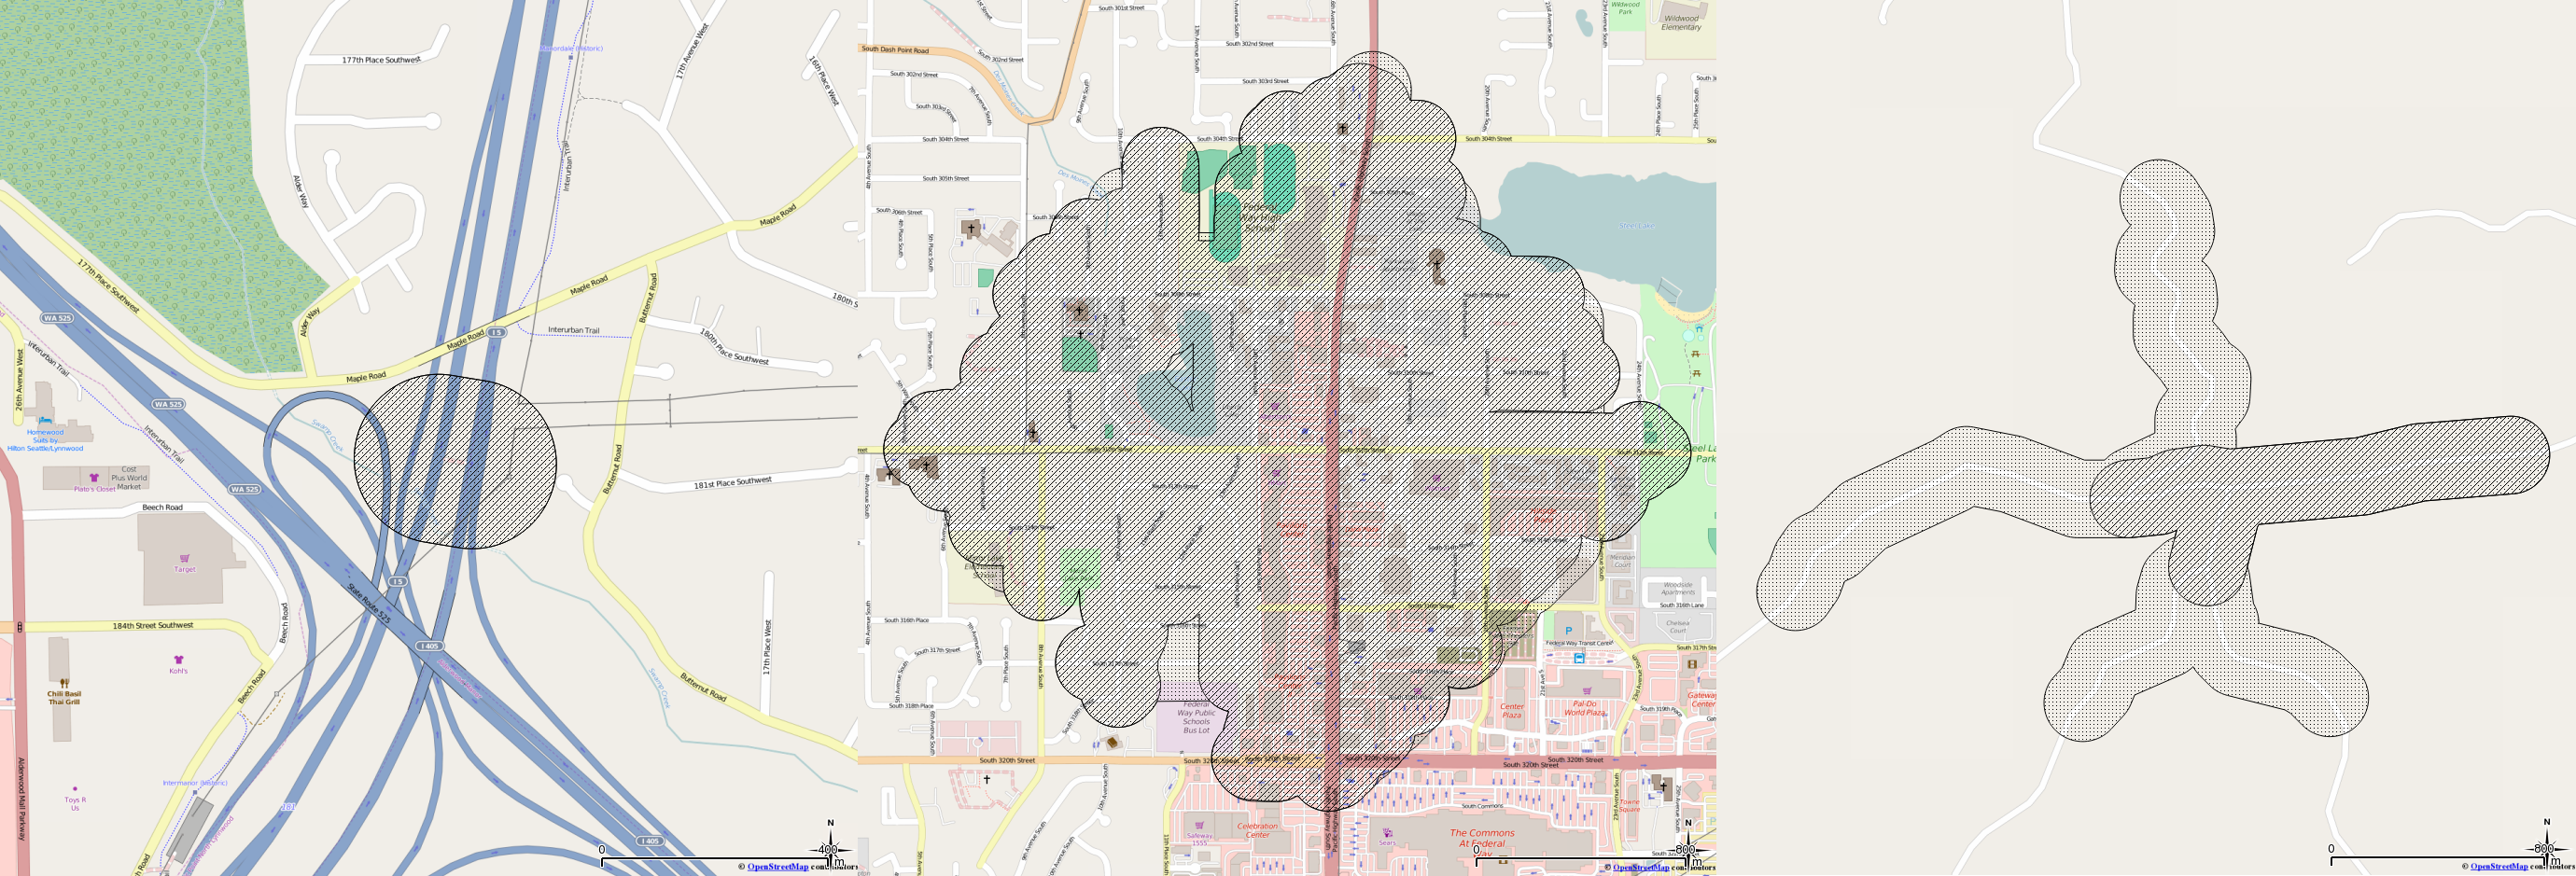
\includegraphics[width=\textwidth]{./figs/symmetric-differences}
  \caption{Three buffers illustrating range of symmetric
    differences. From left to right: buffer with smallest difference,
    buffer with difference nearest the median, and buffer with largest
    symmetric difference. PostGIS buffered regions are denoted by
    diagonal crosshatching, while ESRI buffered regions are
    dot-shaded.}
  \label{fig:symmetric_differences}
\end{figure}

We believe that the primary source of differences between our PostGIS
and ESRI generated buffers to be the result of topological differences
and errors in the network dataset.  As discussed in the methods
section, we imported Open Street Map data into PostGIS in such a way
as to preserve the network topology. Thus, calculations performed with
PostGIS / PgRouting will account for non-apparent discontinuities,
such as where a bridge crosses over another facility in 3d space.

The network used for creation of buffers in ArcGIS, on the other hand,
was the result of constructing a network dataset from a shapefile
exported from PostGIS. Because shapefiles do not preserve topology,
ArcGIS is forced to infer topology. Thus, in our hypothetical
situation where a bridge crosses over another facility, the
reconstructed network may erroneously connect between the bridge and
the road below. In that case, we would expect to see a smaller PostGIS
buffer and a larger ESRI buffer, due to the greater network
connectivity in the ESRI case. While the mean difference in area
between our two sets of buffers was not significant in the statistical
sense, the observed differences in our sample are consistent with the
logic that the more connected, inferred network topology would yield
larger buffers.

Our worst case buffer pair suggests an an extreme version of this size
bias with respect to network topology---namely that potential
topological errors in the Open Street Maps data could be corrected
when imported into ArcGIS via a shapefile. These two buffers are
located in a remote portion of Central Washington, where we might
expect network topology errors to go uncorrected, in this instance
resulting in a false discontinuity. In such instances, the PostGIS
buffer would again be smaller than the ArcGIS buffer. Finally, while
most of the PostGIS-generated buffers were smaller, about 15 percent
were larger than their ESRI-generated sibling, suggesting that
inferred topologies may not always be more connected than the topology
present in the OSM data.

\section*{Conclusions}
This paper set out to validate, in a fully reproducible way, the
sausage buffer approach to creating network-based travel catchment
geographies. We accomplished this by developing procedures using the
PostgreSQL relational database with PostGIS and PgRouting
extensions. We conclude that the sausage buffering method is indeed a
valid and replicable approach to generating network-based travel
catchments, and that PostgreSQL, PostGIS, and PgRouting are 
suitable and offer important benefits for these purposes.

The sausage buffering procedures presented here achieve a higher
standard of reproducibility than previously published sausage
buffering research, in that these are explicitly designed to allow for
automated analyses that are less subject to human error. In addition
to our procedures being fully automated through computer code, the
free and open source nature of PostgreSQL, PostGIS, and PgRouting
confer further benefits to reproducibility. Whereas the true
implementation of ESRI's network analyst is not known outside of ESRI,
all of PgRouting's distance calculations can be scrutinized
directly. Indeed, had the service area calculations in ArcGIS been
fully transparent in this manner, \citeauthor{Forsyth2014sausage} may
not have had cause to develop sausage buffers in the first place.

In addition to establishing a reproducible method for creating sausage
buffers, we also conclude that the sausage buffers created via PostGIS
are generally comparable to sausage buffers created by
ArcGIS. Differences between sausage buffers created in the two
programs are more likely to be due to differences in how network
datasets are constructed, than to differences in how the buffers are
computed.

\printbibliography


\end{document}
